\documentclass[12pt, a4paper, english, singlespacing, parskip]{scrartcl}

%\documentclass[
%11pt, 				% The default document font size, options: 10pt, 11pt, 12pt
%oneside, 			% Two side (alternating margins) for binding by default, uncomment to switch to one side
%chapterinoneline,	% Have the chapter title next to the number in one single line
%english, 			% ngerman for German
%singlespacing, 	% Single line spacing, alternatives: onehalfspacing or doublespacing
%draft, 			% Uncomment to enable draft mode (no pictures, no links, overfull hboxes indicated)
%nolistspacing, 	% If the document is onehalfspacing or doublespacing, uncomment this to set spacing in lists to single
%liststotoc, 		% Uncomment to add the list of figures/tables/etc to the table of contents
%toctotoc, 			% Uncomment to add the main table of contents to the table of contents
%parskip, 			% Uncomment to add space between paragraphs
%nohyperref, 		% Uncomment to not load the hyperref package
%headsepline, 		% Uncomment to get a line under the header
%]{scrartcl or scrreprt or scrbook} % The class file specifying the document structure

\usepackage{amssymb, amsmath, color, graphicx, float, setspace, tipa}
\usepackage[utf8]{inputenc} 
\usepackage[english]{babel}
\usepackage[pdfpagelabels,pdfstartview = FitH,bookmarksopen = true,bookmarksnumbered = true,linkcolor = black,plainpages = false,hypertexnames = false,citecolor = black, breaklinks]{hyperref}
\usepackage{url}
\usepackage{caption}
\captionsetup{font=small,labelfont=bf, format=plain, justification=centering}
\allowdisplaybreaks 		% allows page breaks in align/equation environment

\usepackage{authblk} 		% titlepage stuff
\usepackage[titletoc, title]{appendix}



%--------------------------------------------
% NEW COMMANDS
%--------------------------------------------

\newcommand{\corresponds}{\mathrel{\widehat{=}}}		% equals with hat

\newcommand {\arctanh}{\mathrm{arctanh}}				% Atanh
\newcommand{\arccot}{\mathrm{arccot }}					% Acotanh

\newcommand{\limz}[1]{\lim\limits_{#1 \rightarrow 0}}	% Limes of something towars zero

\newcommand{\bm}{\boldmath}								% Bold font in math
\newcommand{\dps}{\displaystyle}						

\newcommand{\e}{\mbox{e}}								% e noncursive in math mode

\newcommand{\del}{\partial}								% partial diff operator
\newcommand{\de}{\mathrm{d}}							% differential d
\newcommand{\D}{\mathrm{d}}								% differential d
\newcommand{\GRAD}{\mathrm{grad}\ }						% gradient
\newcommand{\DIV}{\mathrm{div}\ }						% divergence
\newcommand{\ROT}{\mathrm{rot}\ }						% rotation

\newcommand{\CONST}{\mathrm{const.\ }}					% constant
\newcommand{\var}{\mathrm{var}}							% variance

\newcommand{\g}{^\circ}									% degrees
\newcommand{\degr}{^\circ}								% degrees

\newcommand{\msol}{M_\odot}								% solar mass


\newcommand{\x}{\mathbf{x}}								% x vector
\newcommand{\xdot}{\dot{\mathbf{x}}}					% x dot vector
\newcommand{\xddot}{\ddot{\mathbf{x}}}					% x doubledot vector
\newcommand{\R}{\mathbf{r}}								% r vector
\newcommand{\rdot}{\dot{\mathbf{r}}}					% r dot vector
\newcommand{\rddot}{\ddot{\mathbf{r}}}					% r doubledot vector
\newcommand{\vel}{\mathbf{v}}							% v vector
\newcommand{\V}{\mathbf{v}}								% v vector
\newcommand{\vdot}{\dot{\mathbf{v}}}					% v dot vector
\newcommand{\vddot}{\ddot{\mathbf{v}}}					% v doubledot vector

\newcommand{\dete}{\mathrm{d}t}							% dt
\newcommand{\delte}{\del t}								% partial t
\newcommand{\dex}{\mathrm{d}x}							% dx
\newcommand{\delx}{\del x}								% partial x
\newcommand{\der}{\mathrm{d}r}							% dr
\newcommand{\delr}{\del r}								% partial r

\newcommand{\deldt}{\frac{\del}{\del t}}				% shortcut partial derivative, in line
\newcommand{\ddt}{\frac{\de}{\de t}}					% shortcut total derivative, in line
\newcommand{\DELDT}[1]{\frac{\del  #1}{\del t}}			% shortcut partial derivative, on fraction
\newcommand{\DDT}[1]{\frac{\de  #1}{\de t}}				% shortcut total derivative, on fraction

\newcommand{\deldx}{\frac{\del}{\del x}}				% shortcut partial derivative, in line
\newcommand{\ddx}{\frac{\de}{\de x}}					% shortcut total derivative, in line
\newcommand{\DELDX}[1]{\frac{\del  #1}{\del x}}			% shortcut partial derivative, on fraction
\newcommand{\DDX}[1]{\frac{\de  #1}{\de x}}				% shortcut total derivative, on fraction

\newcommand{\deldr}{\frac{\del}{\del r}}				% shortcut partial derivative, in line
\newcommand{\ddr}{\frac{\de}{\de r}}					% shortcut total derivative, in line
\newcommand{\DELDR}[1]{\frac{\del  #1}{\del r}}			% shortcut partial derivative, on fraction
\newcommand{\DDR}[1]{\frac{\de  #1}{\de r}}				% shortcut total derivative, on fraction


\newcommand{\U}{\mathbf{U}}                             % state vector
\newcommand{\F}{\mathbf{F}}                             % flux tensor
\newcommand{\half}{\tfrac{1}{2}}

% quickly insert a figure without a caption
% usage: \quickfig{filename}{label}
\newcommand{\quickfig}[2]{
	\begin{figure}[H]
		\includegraphics[width=\textwidth]{#1}
		\caption{\label{#2}}
	\end{figure}
}


% replace \sum with \sum\limits
\let\oldsum\sum
\renewcommand{\sum}{\oldsum\limits}




%-----------------------------------------------
% FORMAT TITLE
%-----------------------------------------------


% Set fonts of document parts
\setkomafont{title}{\rmfamily\bfseries\boldmath}
\addtokomafont{section}{\rmfamily\bfseries\boldmath}
\addtokomafont{subsection}{\rmfamily\bfseries\boldmath}
\addtokomafont{subsubsection}{\rmfamily\bfseries\boldmath}
\addtokomafont{disposition}{\rmfamily} % table of contents and stuff
\setkomafont{descriptionlabel}{\rmfamily\bfseries\boldmath}

\usepackage{grffile}


%------------------------------------------
%: Metadata
%------------------------------------------

\title{Mesh Hydrodynamics Results}
\author{Mladen Ivkovic}
\affil{Laboratory of Astrophysics \\ \'Ecole Polytechnique F\'ed\'erale de Lausanne}
\date{\today}

%------------------------------------------











\begin{document}
	
%--------------------------------------------
% Stuff that needs to be done before all else
%--------------------------------------------
%\pagestyle{plain}
%\nocite{*} % show all entries of bibliography, even if they are not cited.




	


%Titlepage
\maketitle
\newpage
\tableofcontents
\newpage






\newpage
\section{Notation}


We are working on numerical methods.
Both space and time will be discretized.

Space will be discretized in cells which will have integer indices to describe their position.
Time will be discretized in fixed time steps, which may have variable lengths.
Nevertheless the time progresses step by step.

The lower left corner has indices $(0, 0)$ in 2D.
In 1D, index 0 also represents the leftmost cell.




We have:
\begin{itemize}
	\item integer subscript: Value of a quantity at the cell, i.e. the center of the cell. Example: $\U_i$, $\U_{i-2}$ or $\U_{i, j+1}$ for 2D.
	\item non-integer subscript: Value at the cell faces, e.g. $\F_{i-\half}$ is the flux at the interface between cell $i$ and $i-1$, i.e. the left cell as seen from cell $i$.
	\item integer superscript: Indication of the time step. E.g. $\U ^ n$: State at timestep $n$
	\item non-integer superscript: (Estimated) value of a quantity in between timesteps. E.g. $\F^{n + \half}$: The flux at the middle of the time between steps $n$ and $n + 1$.
\end{itemize}
\newpage
\section{Advection}

\subsection{Analytical Equation}

Advection is a bit of an exception as a hydrodynamics method because we're not actually solving the (ideal) gas equations, but these instead:

\begin{equation}
	\DELDT{ \U } + v \cdot \DELDX{\U} = 0
\end{equation}


Which is still a conservation law of the form

\begin{equation}
	\DELDT{ \U } + \DELDX{\F} = 0
\end{equation}

with the flux tensor 

\begin{equation}
	\F = v \cdot \U
\end{equation}

We assume the advection velocity $v = $ const.

Note that in the formalism used, we only solve the 1D advection, but for every component of the state vector $\U$ and flux tensor $\F$

The analytical solution is given by any function $q(x)$ with $\U(x,t) = q(x - v t)$, which is just $q(x)$ translated by $v t$.




\subsection{Piecewise Constant Method}

\begin{figure}[htbp]
	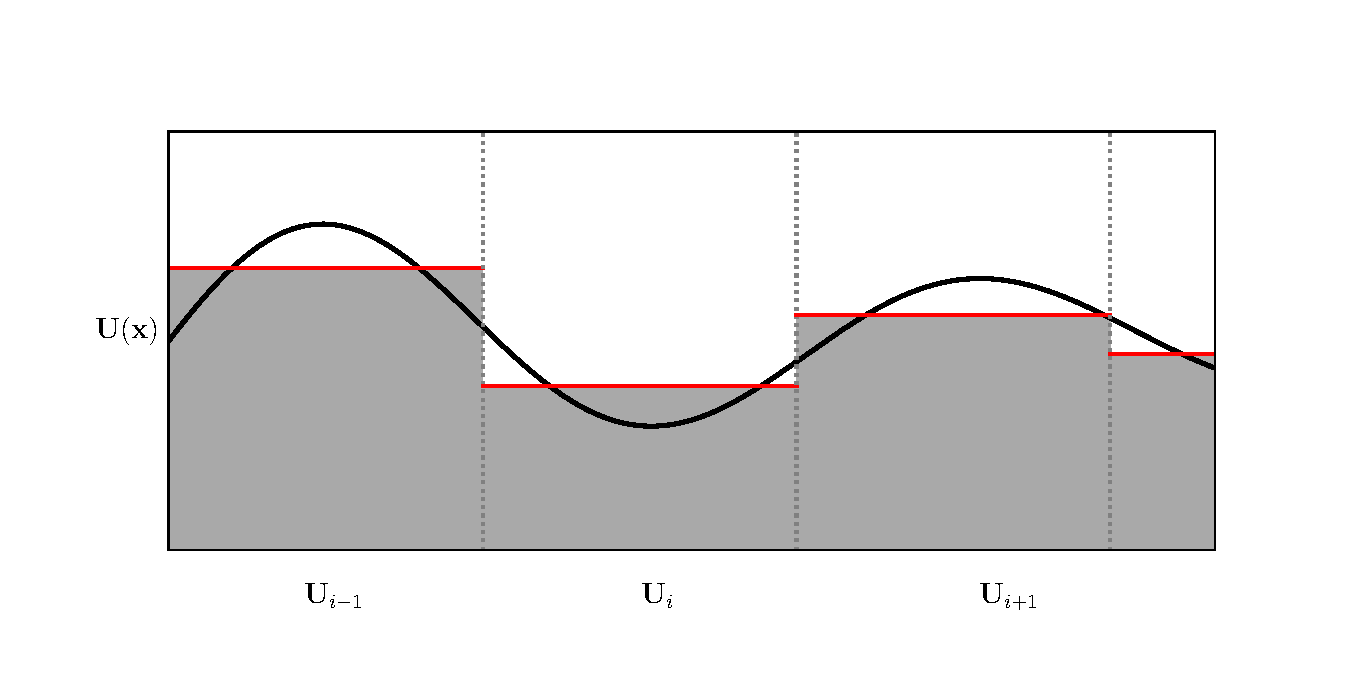
\includegraphics[width=\textwidth]{./figures/piecewise_const.pdf}%
	\caption{Piecewise constant reconstruction of the field
		\label{fig:pwconst}
	}
\end{figure}


We assume that the cell state within a cell is constant (fig. \ref{fig:pwconst}).
Furthermore, we also assume that the velocity $v$ is constant and positive.


\begin{align}
	\U_i ^{n+1} &= 
		\U_i^{n} +  \frac{\Delta t}{\Delta x} \left( \F_{i-\half}^{n+\half} - \F_{i+\half}^{n+\half} \right) \label{eq:advection_basic}\\ 
	\F_{i\pm\half}^{n+\half} &= v_{i\pm\half}\cdot \U_{i - \half \pm \half} \label{eq:advection_flux}
\end{align}

The method is first order accurate in time and space.





We assumed that the velocity is positive and constant.
What if it's negative?

The important point is that we always do \textbf{downwind differencing}.
To obtain a finite difference, as we do here, you must never use the value that is downstream, i.e. that is in the direction of the flux.
Doing this means taking a value for your computation that won't be valid as soon as an infinitesimal time interval passes, because the ingoing flux will change the downwind state.
This is unphysical and leads to violent instabilites.

So if we have negative velocity, all we need to do is change the expression \ref{eq:advection_flux} to

\begin{equation}
	\F_{i\pm\half}^{n+\half} = v_{i\pm\half}\cdot \U_{i + \half \pm \half}
\end{equation}









\subsection{Piecewise Linear Method}

\begin{figure}[htbp]
	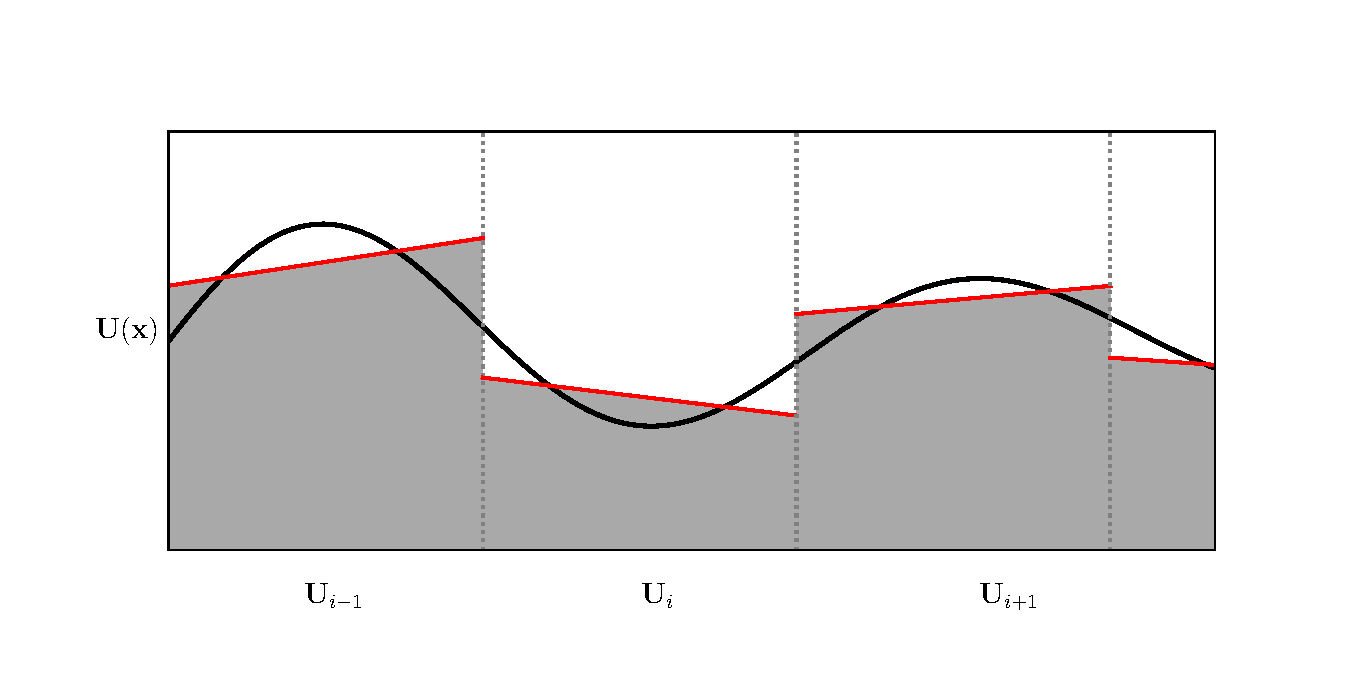
\includegraphics[width=\textwidth]{./figures/piecewise_linear.pdf}%
	\caption{Piecewise linear reconstruction of the field
		\label{fig:pwlin}
	}
\end{figure}



This time, we assume that the state is not constant within a cell, but follows a piecewise linear profile with some slope $\mathbf{s}$ (fig. \ref{fig:pwlin}):

\begin{align*}
	\text{For } x_{i-\half} < x_i < x_{i+\half}: &&
	\quad \U(x, t=t_n) &= \U_i^n + \mathbf{s}_i^n(x - x_i) \\
	\text{Centered method:} && \mathbf{s_i}^n &= \frac{\U_{i+1}^n - \U_{i-1}^n}{ 2 \Delta x}
\end{align*}

Other choices for the slope are possible and stable.




Assuming a positive constant velocity $v$, we derive the flux $\F$ at the time $t^n < t < t^{n+1}$ at the interface position $i-\half$.
At time $t$, the cell will have been advected by a distance $v (t - t^n)$, and the the current state at the interface will be

\begin{align*}
	\U(x=x_{i-\half}, t) 
		&= \U_{i-1}^n + \mathbf{s}_{i-1} (x_{i-\half} - v (t - t^n) - x_{i-1}) \\
		&= \U_{i-1}^n + \mathbf{s}_{i-1} (\frac{1}{2} \Delta x - v (t - t^n))
\end{align*}

To understand how the $x_{i-\half} - v (t - t^n)$ comes into play, imagine the state doesn't change (i.e. isn't advected), but you move the boundaries to the left instead over a distance $v(t - t^n)$.

So if we have a \textbf{negative} constant velocity, the term changes to 

\begin{align*}
	\U(x=x_{i-\half}, t) 
		&= \U_{i}^n + \mathbf{s}_{i} (x_{i-\half} - v (t - t^n) - x_{i}) \\
		&= \U_{i}^n + \mathbf{s}_{i} (-v (t - t^n) - \Delta x)
\end{align*}



Note that the minus sign remains, and that the indices changed by one because we need to always make sure to do upwind differencing, i.e. take only values where the flow comes from, not from the direction where it's going.

Finally, we can compute the average flux over the time step $\Delta t = t^{n+1} - t^{n}$:
\begin{align}
	\F_{i-\half}^{n+\half} 
	&= \langle \F_{i+\half}(t)\rangle _{t^n} ^ {t^{n+1}} 
	= \frac{1}{\Delta t} \int_{t^n}^{t^{n+1}} v \U(x 
	= x_{i-\half}, t) \\
	&= \frac{1}{\Delta t} \int_{t^n}^{t^{n+1}} v \left( \U_{i-1}^n + \mathbf{s}_{i-1} (\frac{1}{2} \Delta x - v (t - t^n)) \right) \\
	&= v \left( \U_{i-1}^n  + \mathbf{s}_{i-1} \left( \frac{1}{2} \Delta x - v \left( \left[ \frac{1}{2 \Delta t} t^2 \right]_{t^n}^{t^{n+1}} - t^n \right)  \right) \right) \\
	&= v \left( \U_{i-1}^n  + \mathbf{s}_{i-1} \left( \frac{1}{2} \Delta x - v \left[ \frac{1}{2} (t^{n+1} + t^n) - t^n \right] \right) \right) \\
	&= v \left( \U_{i-1}^n  + \frac{1}{2} \mathbf{s}_{i-1} \left(\Delta x - v \Delta t \right) \right)
\end{align}



Finally averaging the fluxes over a time step gives:
\begin{equation}
	\U_i^{n+1} = \U_i^n - v \cdot \frac{\Delta t}{\Delta x} ( \U_i ^n - \U_{i-1}^n) - v \cdot \frac{\Delta t}{\Delta x} \frac{1}{2} (\mathbf{s}_i^n - \mathbf{s}_{i-1}^n)(\Delta x - v \Delta t)
\end{equation}

This is the same as eq. \ref{eq:advection_basic} where we used
\begin{align*}
	\F_{i + \half}^{n+\half} 
		& = v_{i+\half} \cdot  \U_{i+\half} ^{n + \half} \\
		& = v \cdot \U(x_{i+\half} - \frac{1}{2} v \Delta t) \\
		& = v \cdot \left( \U_i^n + \mathbf{s}_i^n [(x_{i+\half} - \frac{1}{2} v \Delta t) - x_i ]  \right)\\
		& = v \cdot \left( \U_i^n + \frac{1}{2} \mathbf{s}_i^n (\Delta x -  v \Delta t)  \right)\\
\end{align*}

and analoguely
\begin{align*}
	\F_{i - \half}^{n+\half} 
		& = v \cdot \left( \U_{i-1}^n + \frac{1}{2} \mathbf{s}_{i-1}^n (\Delta x -  v \Delta t)  \right)\\
\end{align*}








To summarize the formulae:

\begin{align*}
	\U_i ^{n+1} &= 
		\U_i^{n} +  \frac{\Delta t}{\Delta x} \left( \F_{i-\half}^{n+\half} - \F_{i+\half}^{n+\half} \right) & \\
	\F_{i-\half}^{n+\half} &= 
		\begin{cases}
			v_{i-\half} \cdot \U_{i-1}^n +  \frac{1}{2} v_{i-\half} \cdot\mathbf{s}_{i-1}^n (\Delta x -  v_{i-\half} \Delta t)
			 	& \quad \text{for } v \geq 0 \\
			v_{i-\half} \cdot \U_{i}^n -\frac{1}{2} v_{i-\half} \cdot \mathbf{s}_{i}^n (\Delta x + v_{i-\half} \Delta t)
				& \quad \text{for } v \leq 0 \\
		\end{cases} \\
	\F_{i+\half}^{n+\half} &= 
		\begin{cases}
			v_{i+\half} \cdot \U_{i}^n +  \frac{1}{2} v_{i+\half} \cdot\mathbf{s}_{i}^n (\Delta x -  v_{i+\half} \Delta t)
			 	& \quad \text{for } v \geq 0 \\
			v_{i+\half} \cdot \U_{i+1}^n -\frac{1}{2} v_{i+\half} \cdot \mathbf{s}_{i+1}^n (\Delta x + v_{i+\half} \Delta t)
				& \quad \text{for } v \leq 0 \\
		\end{cases} \\		
\end{align*}





We can now insert a more general expression for the slopes.
Let 
\begin{align}
	\theta_{i-\half} = \begin{cases} +1 \quad \text{ for } v \geq 0 \\ -1 \quad  \text{ for } v \leq{0} \end{cases}
\end{align}

Then

\begin{align}
	\Delta x_{i-\{0, 1\}} \mathbf{s}_{i-\{0,1\}} 
		&= \frac{1}{2} \Delta x \left[ (1 + \theta_{i-\half}) \mathbf{s}_{i-1}^n + (1 - \theta_{i-\half})  \mathbf{s}_{i}^n \right]  \\
	&\equiv \phi(r_{i-\half}^n) (\U_i^n - \U_{i-1}^n ) \\
	r^n_{i-\half} &= \begin{cases}
		\frac{\U_{i-1}^n - \U_{i-2}^n}{\U_{i}^n - \U_{i-1}^n} 	\quad \text{ for } v  \geq 0 \\
		\frac{\U_{i+1}^n - \U_{i}^n}{\U_{i}^n - \U_{i-1}^n} 	\quad \text{ for } v  \leq 0 \\
	\end{cases} 
\end{align}

$\phi$ is discussed later. Finally:

\begin{align}
	\F_{i-\half}^{n+\half} = 
		&\frac{1}{2} v_{i-\half} \left[  (1 + \theta_{i-\half}) \U_{i-1}^n + (1 - \theta_{i-\half})  \U_{i}^n \right] +\nonumber\\
		&\frac{1}{2}| v_{i-\half} | \left( 1 - \left| \frac{v_{i-\half} \Delta t}{\Delta x} \right| \right) \phi(r_{i-\half}^n) (\U_i^n - \U_{i-1}^n ) \label{eq:advection_phi1}\\
	\F_{i+\half}^{n+\half} = 
		&\frac{1}{2} v_{i+\half} \left[  (1 + \theta_{i+\half}) \U_{i}^n + (1 - \theta_{i+\half})  \U_{i+1}^n \right] +\nonumber\\
		&\frac{1}{2}| v_{i+\half} | \left( 1 - \left| \frac{v_{i+\half} \Delta t}{\Delta x} \right| \right) \phi(r_{i+\half}^n) (\U_{i+1}^n - \U_{i}^n ) \label{eq:advection_phi2}
\end{align}







Depending on our choice of $\phi$, we can get different slopes. Here for positive velocity only, and for $r = r_{i-\half}$:

\begin{align*}
	\phi(r) & = 0 \rightarrow \mathbf{s}_i = 0 
		&\text{ No slopes; Piecewise constant method.}\\
	\phi(r) & = 1 \rightarrow \mathbf{s}_i = \frac{\U_{i} - \U_{i-1}}{\Delta x} 
		&\text{ Downwind slope (Lax-Wendroff)} \\
	\phi(r) & = r \rightarrow \mathbf{s}_i = \frac{\U_{i-1} - \U_{i-2}}{\Delta x} 
		&\text{Upwind slope (Beam-Warming)} \\
	\phi(r) & = \frac{1}{2} (1 + r) \rightarrow \mathbf{s}_i = \frac{\U_{i} - \U_{i-2}}{2 \Delta x} 
		&\text{ Centered slope (Fromm)} \\
\end{align*}

















\subsection{CFL Condition}

To keep things stable and physical, we must not allow any flux in the simulation to go further than one single cell size.
Otherwise, you're skipping interactions between fluxes on cells.
This time restriction is known as the CFL condition.

In 1D, it's straightforward:

\begin{equation}
	\Delta t_{max} = C_{cfl} \frac{\Delta x}{v_{max}} \label{eq:CFL1D}
\end{equation}

$C_{cfl} \in [0, 1) $ is a user-set factor.
The lower it is, the more precise the results, but the more computations you need to do.

In 2D, it is:
\begin{equation}
	\Delta t_{max} = C_{cfl} \left( \frac{|v_{x,max}|}{\Delta x} +  \frac{|v_{y,max}|}{\Delta y} \right)^{-1} \label{eq:CFL2D}
\end{equation}

This condition is more strict than what one would expect from the restriction based on physical arguments, i.e. not allowing the flux to pass more than one cell, which would be $\Delta t_{max} = C_{cfl} \min \left\{ \frac{\Delta x}{|v_{x,max}|} ,  \frac{\Delta y}{|v_{y,max}|} \right\} $.
It follows from a convergence condition in (von Neumann) stability analysis of the method.

For $N$ dimensions, the condition translates to

\begin{equation}
	\Delta t_{max} = C_{cfl} \left( \sum_{i=1}^{N} \frac{|v_{i,max}|}{\Delta x_i} \right)^{-1}  \label{eq:CFLND}
\end{equation}








\subsection{Implementation Details}


What is implemented is the equation

\begin{equation}
    \DELDT{\U} + v \cdot \DELDX{\U} = 0
\end{equation}


where we assume that the velocity $v$ is constant. 
Therefore, the fluid velocity is never updated, but kept identical to the initial conditions.
The fluxes $\F = v \U$ are computed and sored in \verb|pstate pflux| of each cell.
Only the \textbf{net flux} is stored, i.e. $\F_{i-\half} - \F_{i+\half}$.

You can change that behaviour by removing the \verb|ADVECTION_KEEP_VELOCITY_CONSTANT| macro definition in \verb|defines.h|


%===========================================
\section{Slope and Flux Limiters}
%===========================================







%===================================================
\subsubsection{Effects on linear advection}
%===================================================


\quickfigcap
	{./figures/limiters/limiter_comparison.png}
	{fig:limiters-advection}
	{The effect of different slope limiters on linear advection, applied to piecewise linear advection (eqns \ref{eq:advection}, \ref{eq:advection-slope})}




\begin{itemize}

	\item All limiters except superbee still contain diffusion. You can't get rid of it entirely, but we got rid of the oscillations.
	
	\item The minmod resembles the solution of the piecewise constant advection, but pay attention that this is at much later times!
	
	\item Some limiters flatten continuous maxima. Van leer, then MC, then superbee in order of ascending ``flattening''
	
	\item It's as if superbee tries to produce jump discontinuities
	
	\item For order of convergence study, see figs. \ref{fig:advection-convergence-dx-gaussian} - \ref{fig:advection-convergence-CFL-step}, and discussion in section \ref{chap:advection-conclusions}.

\end{itemize}







%=========================================
\section{Riemann Solvers}
%=========================================



%=========================================
\subsection{Approximate Riemann Solutions}
%=========================================






\quickfigcap
	{./figures/riemann/riemann-approximate-sod_test-0.100.png}
	{fig:riemann-approximate-sod-test}
	{
		The Sod test solved using the exact and approximate Riemann solvers
	}
	

\quickfigcap
	{./figures/riemann/riemann-approximate-sod_test-0.200.png}
	{fig:riemann-approximate-sod-test-later}
	{
		The Sod test solved using the exact and approximate Riemann solvers, at a later time
	}
	




\quickfigcap
	{./figures/riemann/riemann-approximate-sod_test_modified-0.100.png}
	{fig:riemann-approximate-sod-test-modified}
	{
		The modified Sod test solved using the exact and approximate Riemann solvers
	}
	

\quickfigcap
	{./figures/riemann/riemann-approximate-sod_test_modified-0.200.png}
	{fig:riemann-approximate-sod-test-modified-later}
	{
		The modified Sod test solved using the exact and approximate Riemann solvers, at a later time
	}
	



\quickfigcap
	{./figures/riemann/riemann-approximate-left_blast_wave-0.006.png}
	{fig:riemann-approximate-left-blast-wave}
	{
		The left blast wave solved using the exact and approximate Riemann solvers
	}
	

\quickfigcap
	{./figures/riemann/riemann-approximate-left_blast_wave-0.013.png}
	{fig:riemann-approximate-left-blast-wave-later}
	{
		The left blast wave solved using the exact and approximate Riemann solvers, at a later time
	}
	





\quickfigcap
	{./figures/riemann/riemann-approximate-right_blast_wave-0.006.png}
	{fig:riemann-approximate-right-blast-wave}
	{
		The left blast wave solved using the exact and approximate Riemann solvers
	}
	

\quickfigcap
	{./figures/riemann/riemann-approximate-right_blast_wave-0.013.png}
	{fig:riemann-approximate-right-blast-wave-later}
	{
		The left blast wave solved using the exact and approximate Riemann solvers, at a later time
	}
	




	
	
	
	
%=========================================
\subsection{Conclusions}
%=========================================
	
	
\begin{itemize}

	\item 	The TSRS solver may have trouble with rarefactions, e.g. figs \ref{fig:riemann-approximate-sod-test} - \ref{fig:riemann-approximate-sod-test-modified-later}.
			Which is to be expected, since it assumes that we have two shocks present.
			It deals much better with shocks, e.g. figs \ref{fig:riemann-approximate-left-blast-wave} - \ref{fig:riemann-approximate-right-blast-wave-later}.
	
	\item 	The TRRS solver may have trouble with shocks, e.g. figs \ref{fig:riemann-approximate-left-blast-wave} - \ref{fig:riemann-approximate-right-blast-wave-later}.
			Which is to be expected, since it assumes that we have two rarefactions present.
			It deals much better with rarefactions, e.g. figs \ref{fig:riemann-approximate-sod-test} - \ref{fig:riemann-approximate-sod-test-modified-later}.
			
			
	\item 	It looks like the results get worse over time.
			Compare figs \ref{fig:riemann-approximate-sod-test} vs \ref{fig:riemann-approximate-sod-test-later}, \ref{fig:riemann-approximate-sod-test-modified} vs \ref{fig:riemann-approximate-sod-test-modified-later}, etc.
			But recall that for the Riemann solver, we only solve the solution once, and then sample the solution for a given $x$ and $t$.
			So once the four regions are determined initially, all the solver does is ``smear them out'' while sampling at a later time $t$.
	
\end{itemize}

%=============================================
\section{Godunov's Method}
%=============================================




%==============================================================
\subsection{Solving Riemann Problems using Godunov's Method}
%==============================================================


\quickfigcap
	{./figures/godunov/GODUNOV-left_blast_wave-1D.png}
	{fig:godunov-1}
	{
		Solution to the left blast wave 
		Riemann problem using Godunov's method and various Riemann solvers.
		The black line is the exact solution.
	}

\quickfigcap
	{./figures/godunov/GODUNOV-right_blast_wave-1D.png}
	{fig:godunov-2}
	{
		Solution to the right blast wave 
		Riemann problem using Godunov's method and various Riemann solvers.
		The black line is the exact solution.
	}

\quickfigcap
	{./figures/godunov/GODUNOV-sod_test-1D.png}
	{fig:godunov-3}
	{
		Solution to the sod test
		Riemann problem using Godunov's method and various Riemann solvers.
		The black line is the exact solution.
	}

\quickfigcap
	{./figures/godunov/GODUNOV-sod_test_modified-1D.png}
	{fig:godunov-4}
	{
		Solution to the modified sod test
		Riemann problem using Godunov's method and various Riemann solvers.
		The black line is the exact solution.
	}

	




%=======================================================================
\subsection{Solving Vacuum Riemann Problems using Godunov's Method}
%=======================================================================









%==============================================================
\subsection{Order of Convergence Study}
%==============================================================



\quickfigcap
	{./figures/godunov/godunov-convergence-dt-500.png}
	{fig:godunov-convergence-dt}
	{
		Testing the method's convergence with respect to the time step $\Delta t$ on Sod test initial conditions.
		For a fair comparison, both the cell width $\Delta x$ and the number of steps taken are fixed.
		The points are measurements, the lines are a linear fit, with the slope of the line given in the legend for each Riemann solver used in the legend.
	}


\quickfigcap
	{./figures/godunov/godunov-convergence-dx.png}
	{fig:godunov-convergence-dx}
	{
		Testing the method's convergence with respect to the cell width $\Delta x$ on Sod test initial conditions.
		For a fair comparison, the Courant number $C_{CFL}$ and the total number of steps are fixed.
		The points are measurements, the lines are a linear fit, with the slope of the line given in the legend for each Riemann solver used in the legend.
	}
	
\quickfigcap
	{./figures/godunov/godunov-convergence-CFL-10000.png}
	{fig:godunov-convergence-CFL}
	{
		Testing the method's convergence with respect to the Courant number $C_{CFL}$ on Sod test initial conditions.
		The points are measurements, the lines are just connecting them.
		The slope of $\half$ is plotted for comparison, and to demonstrate the deviation from it.
	}























%==============================================================
\subsection{Conclusions}
%==============================================================


\begin{itemize}


	\item 	Similar to the piecewise constant advection, the method is diffusive around sharp jump discontinuities.
			See figs. \ref{fig:godunov-1} - \ref{fig:godunov-4}.


	\item \textbf{Order of Convergence}
	
		\begin{itemize}
			
			\item 	Looking at the time step dependence (fig. \ref{fig:godunov-convergence-dt}), we always get slopes around $\sim 0.5$.
					Considering that a Sod test contains multiple jump discontinuities, this is absolutely as expected if we follow the same argumentation as for linear advection.
					See eq. \ref{eq:advection-error-square-root} and derivation leading up to it for comparison.
					All in all, it remains true that jump discontinuities reduce the order of convergence w.r.t. the time step.
					
			\item 	For the cell width dependence (fig. \ref{fig:godunov-convergence-dx}), we get a remarkable slope of $1.000$ for all solvers.
					Even more remarkable, all the $L1$ norms are identical.
					No approximate solver introduces more or less errors in this test case.
			
			\item 	For the $C_{cfl}$ dependence, we see that it deviates more stronger for higher $C_{CFL}$ from the $0.5$ power law that we get for small $\Delta t$.
					However, it is significantly better than what we get for advection (fig. \ref{fig:advection-convergence-CFL-step}).
					
					Why?
					
					Well, we don't necessarily have constant time steps any more, nor do we have constant velocities.
					It is conceivable that the errors ``correct themselves'' by demanding/allowing a smaller/larger timestep.
					
					What also might decrease the accuracy for high $C_{cfl}$ is that I  don't properly compute the emerging wave speeds, but estimate them;
					So there is a possibility that for high $C_{cfl}$, things are just computed wrongly, i.e. the chosen time step is too large to be stable or accurate.
			
		\end{itemize}
\end{itemize}













%------------
%Bibliography
%------------
%https://www.sharelatex.com/learn/Bibliography_management_in_LaTeX
%\medskip % or: \bigskip to add some space


\printbibliography
%\printbibliography[heading=bibintoc,title={Set some title instead of "References"}]
%if heading=bibintoc: set references in table of contents







\end{document}